\chapter{関連技術}
\label{chap:related_works}

\section{ESP32}

\section{WebAssembly}

WebAssemblyは、Google、Microsoft、MozillaおよびAppleの主導によって開発された仮想命令セットである\cite{webassembly}。
従来、WebブラウザにおいてはECMAScript(JavaScript)が事実上唯一の標準化された実行形式であった。
しかし、ECMAScriptはスクリプト言語({\it scripting language})として設計された言語であり\cite{ecma2018}、実行速度や実行効率といった面で最適化されていない。
そこで、WebAssemblyはWebブラウザにおいて高速で安全な実行が可能な形式として設計された。

\subsection{バイナリフォーマット}

\begin{figure}[htbp]
  \caption{WebAssemblyバイナリフォーマットの構成}
  \label{fig:wasm_module}
  \begin{center}
    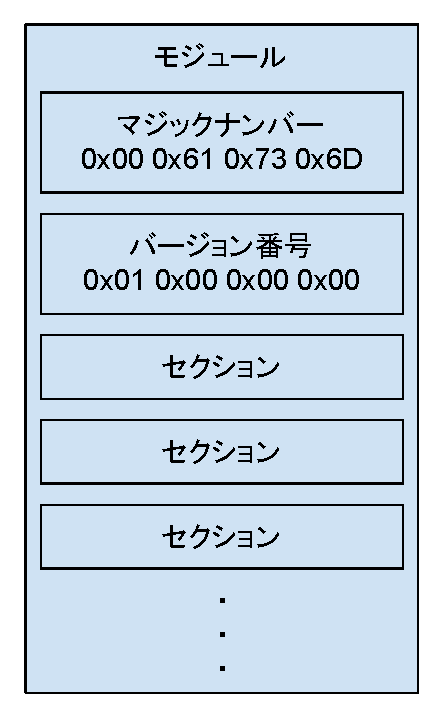
\includegraphics[bb=0 0 800 600,width=12cm]{img/wasm_module.pdf}
  \end{center}
\end{figure}

\paragraph{型}

i32、i64、f32、f64。

\paragraph{関数}

\paragraph{テーブル}

外部の関数への参照テーブルのサイズ情報と型情報。

\paragraph{エレメント}

テーブルを初期化するためのデータ。

\paragraph{メモリ領域}

線形なメモリ領域(ヒープ)のサイズ情報。

\paragraph{データ}

メモリ領域を初期化するためのデータ。

\paragraph{グローバル変数}

グローバル変数の初期値。

\paragraph{インポート}

他のモジュールの型/テーブル/メモリ/グローバル変数への参照。

\paragraph{エクスポート}

他のモジュールへ公開する型/テーブル/メモリ/グローバル変数。

\subsection{検証}

\subsection{実行}

\section{QEMU}

\section{JVM}
